\chapter{Background}
\label{ch:background}

\section{Functional Programming}

Functional programming languages are characterised by the use of first-class functions, higher-order
functions, and the use of recursion instead of loops. These languages are also typically
\emph{referentially transparent}, meaning that the same function call with the same arguments will
always return the same result, regardless of the context in which it is called. This category
of languages can be seen as the application of mathematical functions to programming, with the
language's syntax and semantics being inspired by lambda calculus.

\subsection{Lambda Calculus}

Lambda calculus is a computational model based on the abstraction and application of functions. The
model was introduced by Alonzo Church in the 1930s as a way to formalise the notion of
computability~\autocite{church1936lambda}, and has since been used as a foundation for the design of
functional programming languages. The understanding of procedural languages could also be seen in
terms of lambda calculus~\autocite{landin1965lambda}. The core of lambda calculus consists of three
elements:

\begin{itemize}
    \onehalfspacing
    \item \textbf{Variables}: Representations of values that can be passed to functions.
    \item \textbf{Abstraction}: The process of defining a function by specifying its arguments and
          body.
    \item \textbf{Application}: The process of applying a function to an argument.
\end{itemize}

For instance, the lambda calculus expression \(\lambda x. x + 1\) represents a function that takes
an argument \(x\) and returns \(x + 1\). By nesting lambda abstractions, more complex functions can
be defined. For example, the expression \(\lambda x. \lambda y. x + y\) represents a function that
takes two arguments and returns their sum.

The lambda calculus has the notion of \emph{free} and \emph{bound} variables, where a variable is
bound if it is within the scope of a lambda abstraction, and free otherwise. A function that
contains no free variables are known to be \emph{closed}.

Expressions that are open cannot be evaluated, as they are not fully defined. For instance, the
expression \((\lambda y. x + y)\) is not closed, as the variable \(x\) is free. However, if we
define \(x\) as a constant, or supplied the value of \(x\) in it's enclosing environment, the
expression would be closed and therefore evaluable. A similar concept is seen in programming
languages, where functions that reference variables outside their scope are known as
\emph{closures}. These functions are able to capture the environment in which they were defined and
can be passed around as first-class values.

\section{The Compiler Pipeline}

Compilers play the role of converting a program written in a given programming language into a
corresponding program in a defined target language. While this conversion can theoretically be done
in one step, it is common for compilers to employ multiple phases responsible for each major
transformation of the source code \autocite{grune2012modern}.

\begin{figure}
    \centering
    \includestandalone[width=\textwidth]{Graphics/compiler-pipeline}
    \caption{Simplified view of the phases of a compiler (adapted from \autocite{grune2012modern}).}
    \label{fig:compiler-pipeline}
\end{figure}

As seen in Figure~\ref{fig:compiler-pipeline}, these phases are split into a frontend responsible
for converting the source language into some intermediate representation, and a backend responsible
for converting the given intermediate representation into executable code for the target platform.
This modular approach of dividing the compilation process into phases provides the ability to reuse
certain phases when targeting different platforms, as well as to allow for semantically correct
program optimisations within appropriate phases.

As an example, the Glasgow Haskell Compiler (GHC) makes use of ten mandatory compiler phases
\autocite{ghccompiler}. However, most phases within the GHC are intentionally simple
transformations, leaving the majority of the optimisations to a specific single phase between the
frontend and code generation. Additionally, the GHC is able to select multiple backend targets,
including a C subset, LLVM, and native code generation~\autocite{jones1997transformation}.

\subsection{Lexical Analysis}

During the lexical analysis phase, the source input is converted into a stream of tokens by
identifying meaningful character sequences that can be grouped together. These character sequences,
known as \emph{lexemes}, are associated with a token type indicating whether it is an operator,
identifier, keyword or another feature of the source language. This phase is also responsible for
filtering characters inconsequential to the semantics of a program, such as whitespace and comments.

For instance, the following:

\begin{code}{scala}
    // A simple multiplication
    val x = 4 * 2
\end{code}

\noindent could be converted into the following stream of tokens:

\begin{code}{scala}
    KEYWORD(val) IDENTIFIER(x) EQUALS INTEGER(4) OPERATOR(*) INTEGER(2)
\end{code}

\noindent where \mintinline{scala}{KEYWORD} represents a keyword token,
\mintinline{scala}{EQUALS} represents an equals token, and so on.

A natural mechanism for identifying tokens from a stream of characters is to use regular expressions
\autocite{aho2007compilers}. For instance, the regular expression \texttt{[a-zA-Z]+}
could be used to identify identifiers, while \texttt{[0-9]+} could be used to identify
integers.

\subsection{Syntax Analysis}

The syntax analysis phase, also known as the parsing phase, is responsible for converting the stream
of tokens produced by the lexical analysis phase into a parse tree. This tree represents the
syntactic structure of the lexed tokens, which are derived from a context-free grammar (CFG).
The parse tree is then converted into an abstract syntax tree (AST) by removing nodes that do not
contribute to the semantics of the program, such as those representing parentheses.

While there are a plethora of algorithms and techniques for parsing, the most common method used for
parsing contemporary programming languages as surveyed in 2021 is via a handwritten \emph{recursive
    descent parser} \autocite{eaton2021parser}. This parsing method is based on the idea of a top-down
parser, where the parser starts at the root of the syntax tree and recursively works its way down in
a depth-first, pre-order manner to the leaves of the tree.

Another top-down parsing method are \emph{parser combinators}, which are a form of higher-order
functions that can be used to construct and combine parsers. These combinators provide greater
modularity than recursive descent parsers, as well as the ability to construct parsers that are more
expressive than those that can be constructed by recursive descent.

\subsection{Intermediate Code Generation}

The intermediate code generation phase is responsible for converting the AST produced by the syntax
analysis phase into an intermediate representation (IR) that is closer to the target language. This
IR is typically a low-level representation that is easier to optimise and convert into machine code
than the original source code. The IR is also used to decouple the frontend from the backend of the
compiler, allowing for platform-generic optimisations to be implemented, as well as facilitating the
reuse of the frontend when targeting different platforms.

\section{LLVM IR}

\begin{figure}[b]
    \centering
    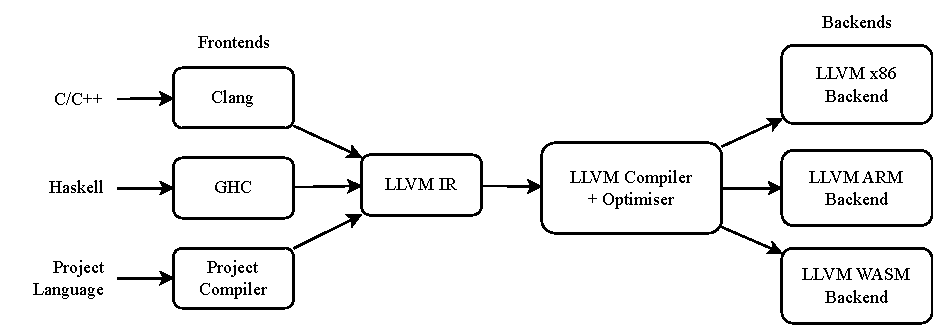
\includegraphics[width=\textwidth]{Graphics/llvm}
    \caption{Integrating the LLVM into a compiler pipeline.}
    \label{fig:llvm}
\end{figure}

The LLVM project is an open-source collection of tools and libraries for the construction of
compilers and related programming tools, the core of which revolves around the LLVM intermediate
representation (LLVM IR). This IR is low-level enough to be used as a target for compilers from
which an LLVM backend can generate machine code, while also being high-level enough to be used as a
portable assembly language targeting a variety of architectures. While originally designed as a
target for compiling C and C++ programs, the LLVM has since been used as a backend for a variety of
languages, including Rust, Swift, and Haskell.

As seen in Figure~\ref{fig:llvm}, targeting the LLVM IR in a compiler pipeline allows for the
compiler to take advantage of the LLVM optimiser, which is capable of performing a variety of
optimisations such as constant propagation, dead code elimination, and loop optimisations. No extra
work is required to target different architectures, as the LLVM backend is capable of generating
machine code for a variety of platforms, including x86, ARM, and even the web via WebAssembly.

From its inception, the IR was designed to be represented in Static Single Assignment (SSA) form
\autocite{lattner2004llvm}, restricting the IR such that each variable must be assigned to exactly
once before usage, and cannot be reassigned. This restriction alone would imply that purely
functional languages could be represented in SSA form, as these languages enforce immutability.
However, the SSA used in LLVM IR also enforces that expressions be atomic, with functions being
strictly applied to only variables or constants, akin to assembly instructions. The effect of this
is that the evaluation order of expressions and program flow is made explicit, simplifying
optimisations such as dead code elimination and constant propagation.

For instance, the following Scala code:

\begin{code}{scala}
    def foo(x: Int, y: Int): Int = x + y * x
\end{code}

could be converted into the following LLVM IR:

\begin{code}{llvm}
    define i32 @foo(i32 %x, i32 %y) {
        %mul = mul i32 %y, %x
        %add = add i32 %x, %mul
        ret i32 %add
    }
\end{code}

Observe that the arithmetic order of operations is made explicit in the LLVM IR, with the
multiplication of \texttt{\%y} and \texttt{\%x} being computed before the addition of \texttt{\%x}
and \texttt{\%mul}. This explicitness allows for the compiler to reorder instructions and perform
optimisations that would not be possible in the original source code.

